\addchap{ASCII - Das Café in der Fakultät}

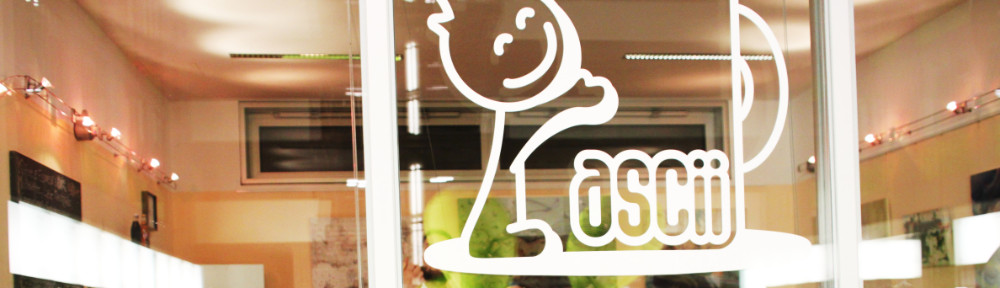
\includegraphics[width=\linewidth]{img/ascii.jpg}

Seit 2007 gibt es in der Fakultät Informatik das ASCII, ein von Studenten betriebenes Café ganz nach der Vorstellung eines richtigen Informatikers.
Es gibt neben diversen Kaffeesorten auch kalte Getränke (Stichwort Mate) und sogar Bagels, Muffins und Donuts, sprich:
alles was ein müder Informatiker morgens braucht, wobei \glqq morgens\grqq\ auch gerne mal 13 Uhr sein kann.
Das ASCII zählt zudem zu den wenigen Adressen auf dem Campus, in denen man Kolle Mate, Club Mate und Premium Cola erhält.
Hinter dem Tresen stehen fast ausschließlich Studenten, die an einem Tag in der Woche noch ein paar Stündchen zur Verfügung stellen können.
Das heißt es werden auch jedes Semester neue Leute gesucht, die gerne mitmachen wollen.

Das ASCII ist seit seiner Gründung zu einer zentralen Anlaufstelle an unserer Fakultät geworden.
Hier treffen sich Studenten, Mitarbeiter und Professoren der Informatik, aber auch Besucher von anderen Fakultäten kommen gerne vorbei um hier ihre Kaffeepausen zu verbringen oder ihren Koffeinhaushalt aufzufüllen.
Auf den gemütlichen Sofas kann man die Zeit wunderbar an sich vorbei streichen lassen, gemeinsam an Projekten arbeiten, lernen, programmieren oder einfach nur mit seinen Kommilitonen plaudern.
Wenn du jetzt Lust bekommen hast, das ASCII auch mal zu besuchen oder sogar als Mitglied selbst hinter dem Tresen zu stehen, dann komm doch einfach mal vorbei und sag hallo!

Das aktuelle Angebot oder Aktuelles erreicht ihr unter \link{http://www.ascii-dresden.de/}.

\textit{Wir öffnen in der Vorlesungszeit Montag bis Donnerstag von 9 bis 17 Uhr und freitags von 9 bis 15 Uhr.}
